\section{Outlook}

\subsection*{State of Art and Future}
\begin{frame}
\begin{columns}[c]
\begin{column}{0.55\textwidth} 
{\bf \center State of Art:}

\quad

\begin{enumerate}
\scriptsize{
 \item Measuring different {\bf NSs (M-R)} can {\bf constrain the EoS} of cold ultradense matter.
 
 \quad
 
 \item  More than 10 years worth of {\bf Rossi X-ray Timing Explorer}(RXTE), the {\bf Chandra X-ray Observatory}, and the {\bf XMM-Newton observations}, with many NSs showing {\bf thermal emission}.
 
 \quad
 
  \item {\bf X-ray bursts}  useful for inferring {\bf NSs (M-R)}, but systematic and statistical errors  {\bf currently do not allow to pin down a unique EoS}. 
  
}
\end{enumerate}
\end{column}

\begin{column}{0.55\textwidth}  
{\bf \center Future Missions and Challenges:}
\begin{enumerate}\scriptsize{
 \item Future observations with {\bf high spectral energy resolution}: {\bf Astro-H}, {\bf ATHENA}.
 

   
 \quad
 
 \item {\bf GAIA} mission will allow {\bf precise measurements of source distances}, constraining $D$ for the radius determination of {\bf thermally emitting stars}.
 
 
 
 \quad
 
 \item Observations of NSs with {\bf  high timing resolution} will be possible with {\bf LOFT} mission.
 
 \quad
 
 \item  {\bf Other approaches to constrain (M-R)} can be explored, e.g. modeling the {\bf pulse profiles} from {\bf non-uniform emission from surface of rotating NSs}, looking for primary {\bf GR effects}.
 

 
 \quad
 
 \item Achieving  {\bf overconstrained measurements} in the EoS allows testing {\bf effects of strong gravitational fields} on NS surfaces.
 }
\end{enumerate}
\end{column}

\end{columns}
\end{frame}





%%%%%%%%%%%%%%%%%%%%%%%%%%%%%%%%%%%%%%%%%%%%%%%%%%%%%%%%%%%%%%%%%%%%%%%%%%%%%%%
%%%%%%%%%%%%%%%%%%%%%%%%%%%%%%%%%%%%%%%%%%%%%%%%%%%%%%%%%%%%%%%%%%%%%%%%%%%%%%%
%%%%%%%%%%%%%%%%%%%%%%%%%%%%%%%%%%%%%%%%%%%%%%%%%%%%%%%%%%%%%%%%%%%%%%%%%%%%%%%
\subsection*{Backup}

\begin{frame}
\frametitle{What are X-ray bursts}
\begin{itemize}\scriptsize{
 \item More than 2000 NSs have been discovered in the Galaxy, from {\bf pulsating sources in radio} to {\bf bright persistent sources in X-Rays}.
 
 \quad
 
 \item They are {\bf bright}.
 
 \quad 
 
 \item We see the {\bf neutron star surface}.
 
 \quad
 
 \item Spectra well fit by {\bf Planck curves}.
 
 \quad
 
 \item {\bf Type I X-ray bursts} to infer {\bf (M,R)}.
 
 \quad
 

\item The large observational catalogues of type I X-ray bursts now available.
}
\end{itemize}
\end{frame}





%%%%%%%%%%%%%%%%%%%%%%%%%%%%%%%%%%%%%%%%%%%%%%%%%%%%%%%%%%%%%%%%%%%%%%%%%%%%%%%%%%%


\begin{frame} 
\begin{columns}[c]
\begin{column}{0.65\textwidth} 
	{\bf \center Radiation of Residual Heat in Young NSs} 
\begin{enumerate}
\scriptsize{
	   \item {\bf After Supernova explosion}: 
	   \begin{itemize}\scriptsize{
	    \item Hot protoneutron star with $T\sim 10^{11} K$;
	    \item Cools by $\nu$ emission from the interior to surface.}
	   \end{itemize}

	   
	   \item {\bf After the supernova explosion}: 
	   \begin{itemize}\scriptsize{
	    \item NS divided into a stellar interior and an outer heat blanketing envelope;
	    \item The interior becomes isothermal within few years.
	    \item The envelope sustains strong $\nabla \textbf{ T}$, is $\sim 100$ m deep, and has short time relaxation, stationary, plane-parallel in hydrostatic equilibrium.
	      \item The thermal evolution of the core (described by the GR solutions of a spherical symmetric star) depends on the heat capacity (degenerate constituents) of the core and neutrino emissivity (composition).}
	   \end{itemize}

	  
	   \item {\bf First 10-100 years}: stellar envelope thermally relaxes by radiating its thermal energy.
	   
	   \quad
	   
	   \item {\bf Following $10^5$ years}: temperature of the crust is set by the temperature of the isothermal core.
	   }
\end{enumerate}	
\end{column}
\begin{column}{0.4\textwidth}    
 \center{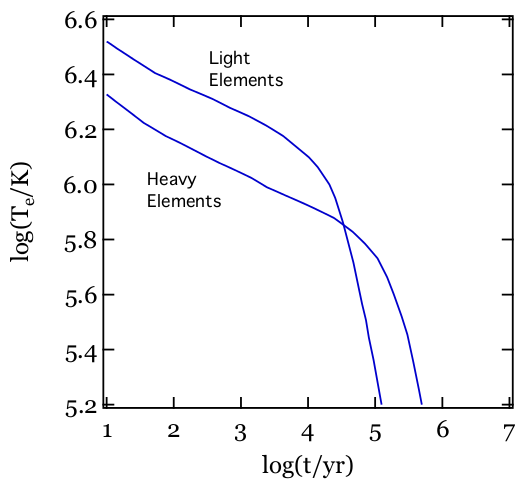
\includegraphics[scale=0.23]{figs/cool.png}}\\
 {\tiny Thermonuclear burst from 4U 1636+536 showing PRE (a) compared to an ordinary burst in panel (b). }
\end{column}
\end{columns}
\end{frame}





%%%%%%%%%%%%%%%%%%%%%%%%%%%%%%%%%%%%%%%%%%%%%%%%%%%%%%%%%%%%%%%%%%%%%%%%%%%%%%%%%%%

\begin{frame}
\begin{columns}[c]
\begin{column}{0.5\textwidth} 
	{\bf \center Reradiation of deposition heat between accretion episodes:}

	
 	{\scriptsize 
	  \begin{itemize}
	   \item Electron capture and pycnocuclear reactions at $\rho \sim 10^{12}$ g cm$^{-3}$ at the crust, releasing $Q_{nuc} \sim 1.5-2$ MeV per accreted baryon.
	   
	   \quad
	   
	   \item A fraction of energy missed by neutrino radiation but some is deposit in the interior, sufficient to power quiescent emission.
	  \end{itemize}
	}    
\end{column}
\begin{column}{0.5\textwidth}  
	{\bf \center Magnetic Field Decay:}
	

 	{\scriptsize 
	  \begin{itemize}
	  \item Decay of strong B $(>10^{14}$ G) releases hot from crust fracturing under stress. {\tiny (Cumming et al 2008, Arras et al, 2004)}
	  
	  \quad
	  
	  \item $E\sim 10^{44}$ erg over hundred section.
	  \end{itemize}
	}   
	\quad
	
		{\bf \center Particle Bombardment onto Polar Caps:}
		
		
 	\scriptsize{ Relativistic electron-positron in the magnetosphere of pulsar bombard the polar caps on the surface, thermal emission peaked in the UV to X-ray. }


\end{column}
\end{columns}
\end{frame}

%%%%%%%%%%%%%%%%%%%%%%%%%%%%%%%%%%%%%%%%%%%%%%%%%%%%%%%%%%%%%%%%%%%%%%%%%%%%%%%%%%%


\begin{frame}

\begin{columns}[c]
\begin{column}{0.5\textwidth} 
	{\bf \center Surface Composition}

\begin{itemize}\scriptsize{ 
 \item Composition of NS determined by: abundance of material during supernova explosion, abundance of material accreted from companion or ISM, gravitational ?? of heavy elements.
 \item Even  light elements like O can remain in the photosphere and give atomic lines on the spectrum  if there is no lighter elements or if its continuously fueled by accretion or convection (short timescale for sedimentation of heavy elements).
 \item The amount of H to cover the surface of a NS down to its photosphere (non B) is
 $$ M_H = 4 \pi R^2 h N_p m_p,$$
 with gas ionized ($N_H=N_p$), which shows to be very small, and the timescale for accretion of sufficient H to cover surface $\ll$ 1 yr to $\sim 10^3$ yr, dominant H and He.}
 \end{itemize}

\end{column}
\begin{column}{0.5\textwidth} 
 
 	{\bf \center  Magnetic Field Strengths}
 \begin{itemize}\scriptsize{ 
  \item From $<10^8$ G to steadying accreting NS to $\sim 10^{15}$ magnetars.
  \item Profound effects on the surface, most important parameter for emission properties.
  \item Affects propagation of photons in the atmosphere, together with polarization of magnetic vacuum (plasma density low)
  \item Photos interact primary  with virtual pairs, vacuum polarization is affected by B, in the presence of a plasma with density gradient (ns atm): resonance on the normal modes of photon propagation, from circular at high e dens (deeper atm) to linear (low densities), so critical density depending on the photon energy, the conversion of photons between the two polarization modes is enhanced, together by chance in the opacities of the normal modes., resonances five rise to broad absorption-like feature. {\tiny (Ozel 2001)}}
 \end{itemize}
 \end{column}
 \end{columns}
\end{frame}




%%%%%%%%%%%%%%%%%%%%%%%%%%%%%%%%%%%%%%%%%%%%%%%%%%%%%%%%%%%%%%%%%%%%%%%%%%%%%%%%%%%




%%%%%%%%%%%%%%%%%%%%%%%%%%%%%%%%%%%%%%%%%%%%%%%%%%%%%%%%%%%%%%%%%%%%%%%%%%%%%%%%%%%


\begin{frame}
\frametitle{Flux and Spectrum of NSs Surface Emission}
\begin{itemize}\scriptsize{ 
 \item Initially the energy is in the crust or core, deeper than atmosphere.
 
 \quad
 
 \item Modeling: assumption of hydrostatic equilibrium, valid if the flux of radiation emitted from the NS does not lead to force $>$ the gravitational force on surface (As long as  the radioactive flux remains below the EL, there is hydrostatic equilibrium).
 
 \quad 
 
 \item Defining {\bf local Eddington limit (EL)} as the luminosity at which radiation balances gravitational forces:
 $L_{Edd} = \frac{8 \pi G M m_p c}{(1+X)\sigma_T}$
 
 \quad
 
\item Very large gravitational acceleration on the NS surface:
$$ g \sim \frac{GM}{R^2} \sim 1.9 \times 10^{14} \Big ( \frac{M}{1.4 M_{cdot}} \Big ) \Big ( \frac{R}{10 m} \Big)^{-2} cm s^{-2}.$$

\item This leads to a very small {\bf scale height} for atmosphere (matter taken as fully ionized):
$$ h \sim 2 \frac{k_BT}{m_p g} \sim 8.8 \Big ( \frac{T}{10^7 K} \Big )  \Big ( \frac{M}{1.4 M_{cdot}} \Big )^{-1} \Big ( \frac{R}{10 m} \Big)^{2} cm.$$

\item Since the scale height $\ll$  NS radius: plane parallel atmosphere in the models.

\quad 


\item 
{\tiny (timescale protons exchange E with matter in photosphere is much shorter than the timescale the interior cools)}

} 
\end{itemize}
\end{frame}



\begin{frame}
\frametitle{Finally, with the right fits...}
\begin{columns}[c]
\begin{column}{0.55\textwidth} 
\begin{center}
  \center{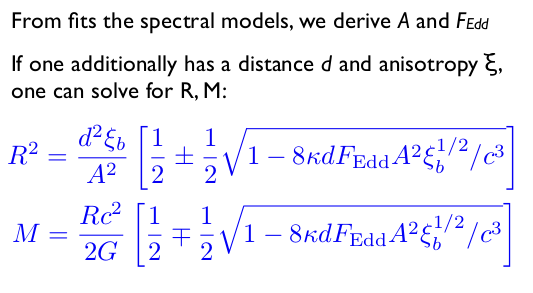
\includegraphics[scale=0.32]{figs/qq.png}}
\end{center}
\end{column}
\begin{column}{0.55\textwidth} 
  \center{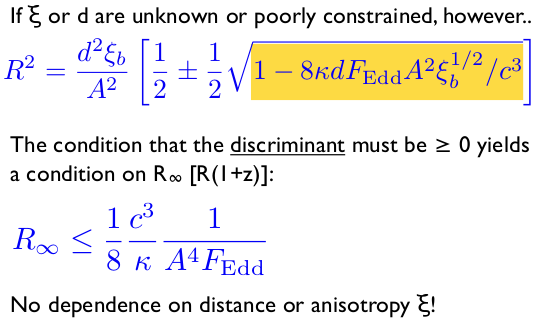
\includegraphics[scale=0.32]{figs/q.png}}
 \end{column}
 \end{columns}

\end{frame}


\begin{frame}
\frametitle{Thermonuclear Bursts (TB)}
	  \begin{enumerate}\scriptsize{ 
	   \item {\bf Recurrent X-ray flashes} with rise time of $\sim 1$ s and duration of $\sim 10$ s  (Type I X-ray bursts, with luminosities up to twice to the {\bf accretion luminosity}).
	   
	   \quad
	   
	      \item Accreting NSs with  {\bf weak B} $(<10^{10}$ G), where {\bf He and H} come from the {\bf binary company}.
	   
	  
	   
	   \quad
	   
	   \item {\bf Several mass accretion rate regimes} leading to thermonuclear flashes with different characteristics. They are typically expressed in units of {\bf Eddington mass accretion rate}:
	  
	  $$\dot M_E = \frac{8 \pi m_p cR}{(1+X)\sigma_T} = 1.8 \times 10^{-8} \Big (\frac{R}{10 \mbox{ km}} \Big ) \Big (\frac{1+X}{1.7}\Big)^{-1} M_{\odot} \mbox{ yr}^{-1}.$$
	  
	where
	  
	  \begin{itemize}\scriptsize{ 
	   \item $\dot m = \dot M/\dot M_E <0.01$: {\bf H burning is unstable and triggers unstable He burning}.
	   \item $0.01< \dot m < 0.1$: {\bf H burns stably into He  between bursts, until He ignites}.
	   \item $0.1< \dot m<0.9$: {\bf He ignites unstably}. }
	  \end{itemize}
}
	  \end{enumerate}
\end{frame}


